\begin{frame}{Methodology}	
	\begin{enumerate}
		\item  The \textbf{cloudSEN12 high-quality dataset} is used only for this experiment $D$; pixel-by-pixel cloud masking is converted to cloud cover percentages in order to perform a regression task.
		\item The dataset of S2 L1C $\{x_1, x_2, ..., x_n\}$ and corresponding cloud cover percentages $\{y_1, y_2, ..., y_n\}$ is splitted in train ($D_{train}$), validation ($D_{val}$), and test ($D_{test}$) dataset.
		\item \textcolor{red}{\textbf{Experiment 01}}: Convolutional Neural Network (CNN) for regression.
	\end{enumerate}
\end{frame}



\begin{frame}{Methodology}	
	\begin{enumerate}
		\item  The \textbf{cloudSEN12 high-quality dataset} is used only for this experiment $D$; pixel-by-pixel cloud masking is converted to cloud cover percentages in order to perform a regression task.
		\item The dataset of S2 L1C $\{x_1, x_2, ..., x_n\}$ and corresponding cloud cover percentages $\{y_1, y_2, ..., y_n\}$ is splitted in train ($D_{train}$), validation ($D_{val}$), and test ($D_{test}$) dataset.		
		\item \textcolor{red}{\textbf{Experiment 02}}: CNN with a GP header layer.
		\begin{itemize}
			\item Residual CNN $f_\theta: x \rightarrow R^J$ with feature space dimensionality $J$ and parameters $\theta$.
			\item Exact GP header with parameters $\phi = \{l, s\}$ where $l$ and $s$ are kernel hyperparameters.			
		\end{itemize}		
	\end{enumerate}
\end{frame}


\begin{frame}{Methodology}
	\begin{enumerate}
		\item  The \textbf{cloudSEN12 high-quality dataset} is used only for this experiment $D$; pixel-by-pixel cloud masking is converted to cloud cover percentages in order to perform a regression task.
		\item The dataset of S2 L1C $\{x_1, x_2, ..., x_n\}$ and corresponding cloud cover percentages $\{y_1, y_2, ..., y_n\}$ is splitted in train ($D_{train}$), validation ($D_{val}$), and test ($D_{test}$) dataset.
		\item \textcolor{red}{\textbf{Experiment 03}}: Variational Deep Kernel Learning.
		\begin{itemize}
			\item Residual NN $f_\theta: x \rightarrow R^J$ with feature space dimensionality $J$ and parameters $\theta$.			
			\item Approximate GP header with parameters $\phi = \{l, s, \omega\}$ where $l$ and $s$ are kernel hyperparameters, $\omega$ GP variational parameters (including $m$ inducing point locations $Z$).
			\item Using a random subset of $p$ points of our training
			data, $X^{init} \subset X$, compute; \textbf{Initial inducing points:} Use found centroids as initial inducing point locations Z in GP. \textbf{Initial length scale:} set
			as 1.			
		\end{itemize}
	\end{enumerate}
\end{frame}


\begin{frame}{Experiment 01}
\begin{figure}
	\centering
	\includegraphics[width=1\linewidth]{images/method_01}
	\caption{}
	\label{fig:method01}
\end{figure}
\end{frame}


\begin{frame}{Experiment 02 - Gaussian processes}
\textbf{\large Definition}

A Gaussian process (GP) is a collection of random variables, any finite number of which have a joint Gaussian distribution.

\textbf{\large Nonparametric Regression Model}
Prior: $f(x) \sim \mathcal{G P}\left(m(x), k\left(x, x^{\prime}\right)\right)$, meaning $\left(f\left(x_{1}\right), \ldots, f\left(x_{N}\right)\right) \sim \mathcal{N}(\boldsymbol{\mu}, K)$, with $\mu_{i}=m\left(x_{i}\right)$ and $K_{i j}=\operatorname{cov}\left(f\left(x_{i}\right), f\left(x_{j}\right)\right)=k\left(x_{i}, x_{j}\right)$.
$$
\overbrace{p(f(x) \mid \mathcal{D})}^{\text {GP posterior }} \propto \overbrace{p(\mathcal{D} \mid f(x))}^{\text {Likelihood }} \overbrace{p(f(x))}^{\text {GP prior }}
$$
	
\begin{figure}
	\centering
	\includegraphics[width=0.75\linewidth]{images/gp01}
	\caption{}
	\label{fig:gp01}
\end{figure}
\end{frame}


\begin{frame}{Experiment 02 - Gaussian processes}
\begin{figure}
	\centering
	\includegraphics[width=0.75\linewidth]{images/gp02}
	\caption{}
	\label{fig:gp01}
\end{figure}
\end{frame}


\begin{frame}{Experiment 02 - Gaussian processes}
	\begin{figure}
		\centering
		\includegraphics[width=0.75\linewidth]{images/gp03}
		\caption{}
		\label{fig:gp01}
	\end{figure}
\end{frame}

\begin{frame}{Experiment 02 - Gaussian processes}
	\begin{figure}
		\centering
		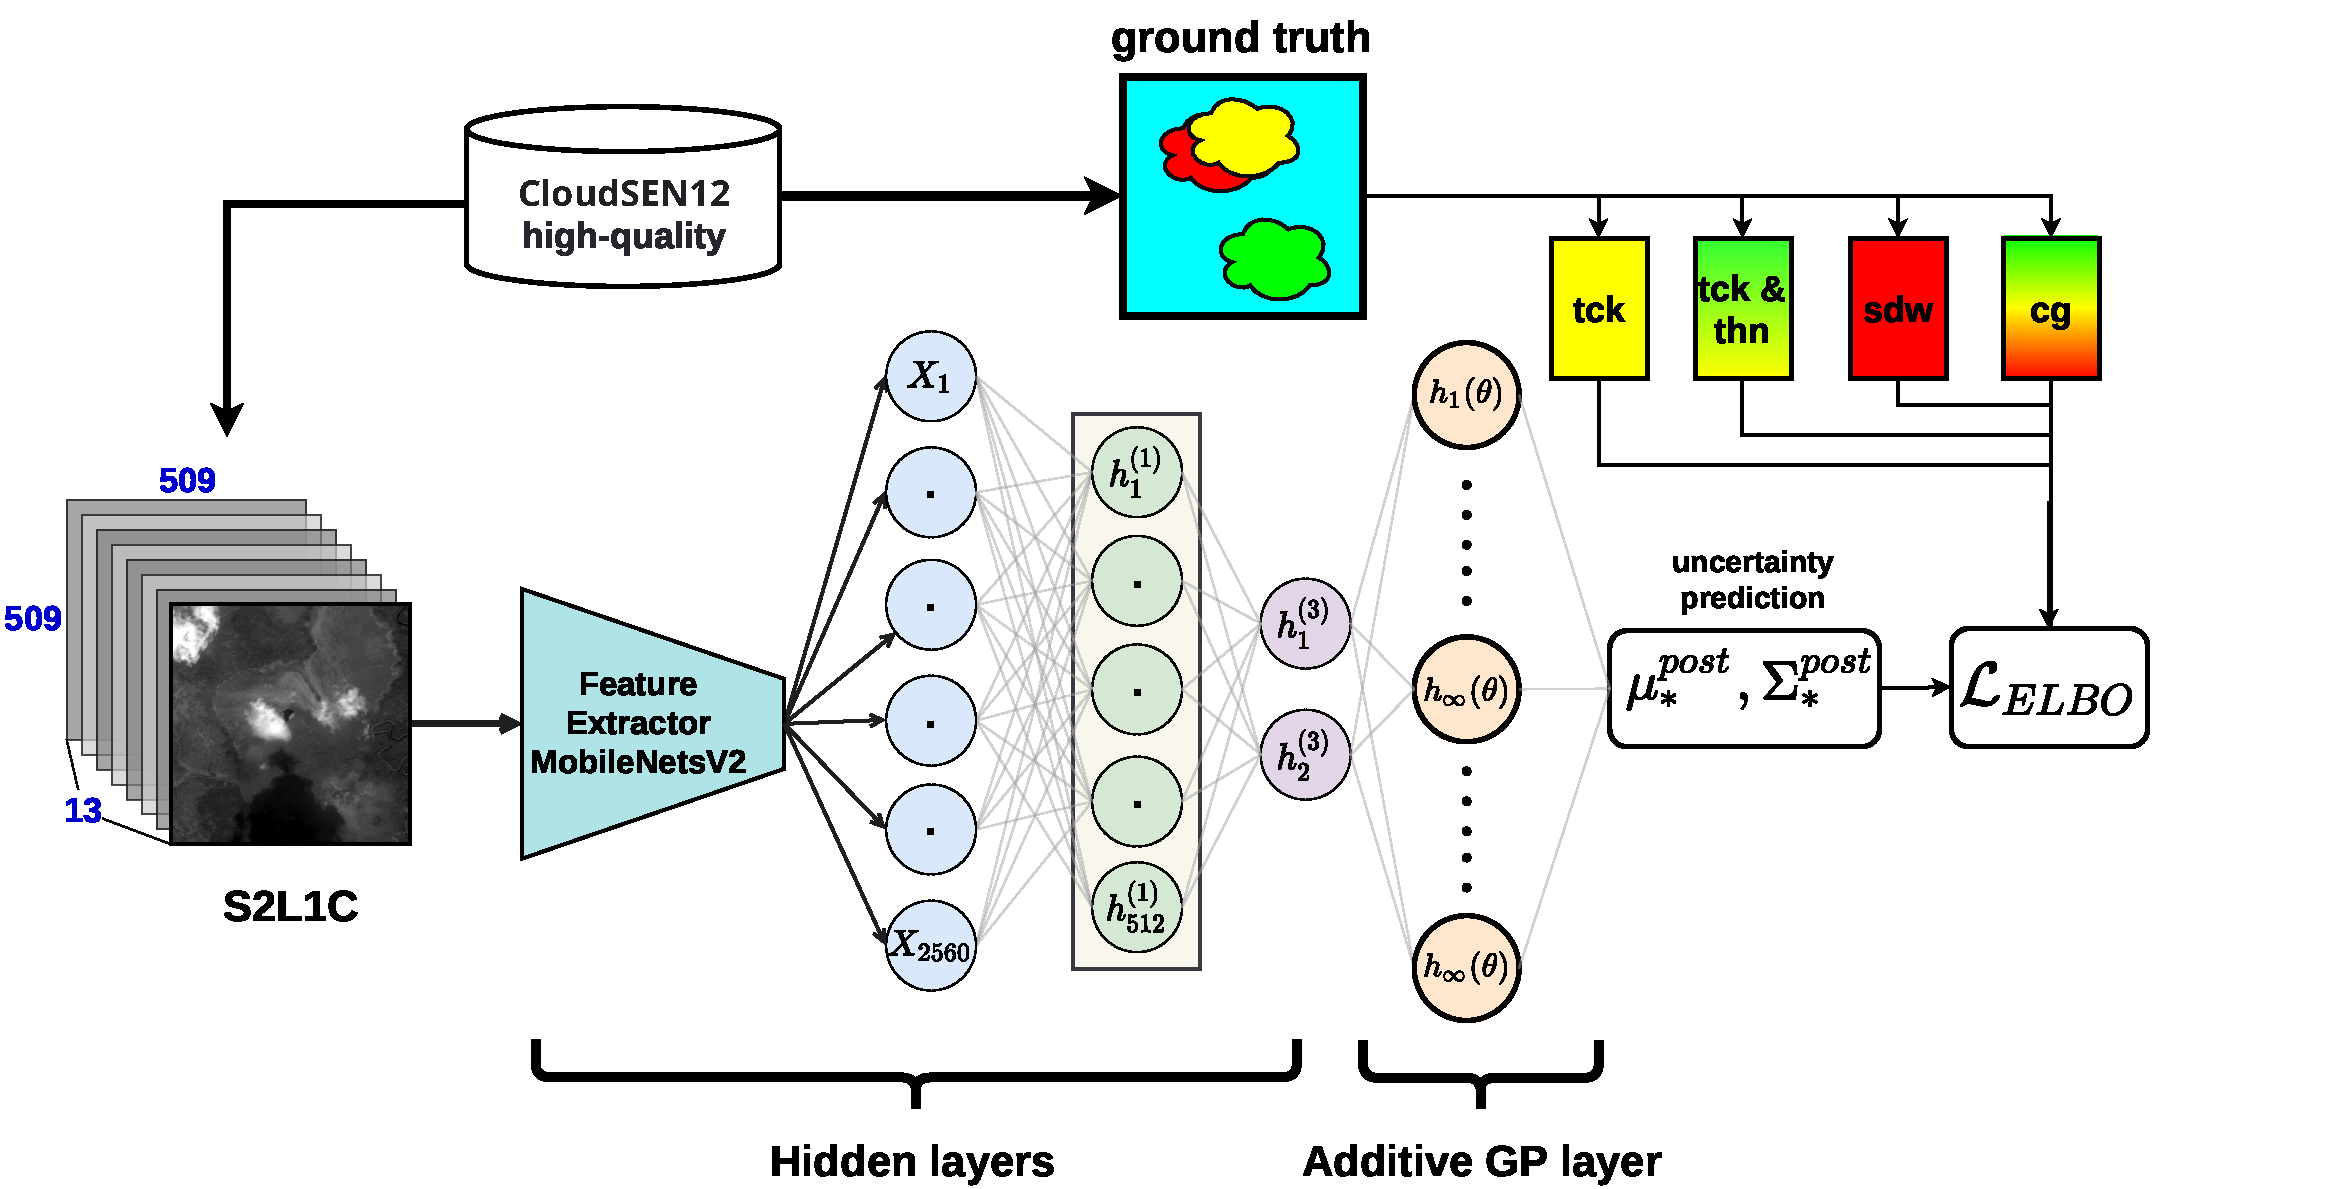
\includegraphics[width=1\linewidth]{images/metodology.pdf}
		\caption{}
		\label{fig:gp01}
	\end{figure}
\end{frame}



\begin{frame}{Experiment 03 - Stochastic Variational DKL}
	\begin{figure}
		\centering
		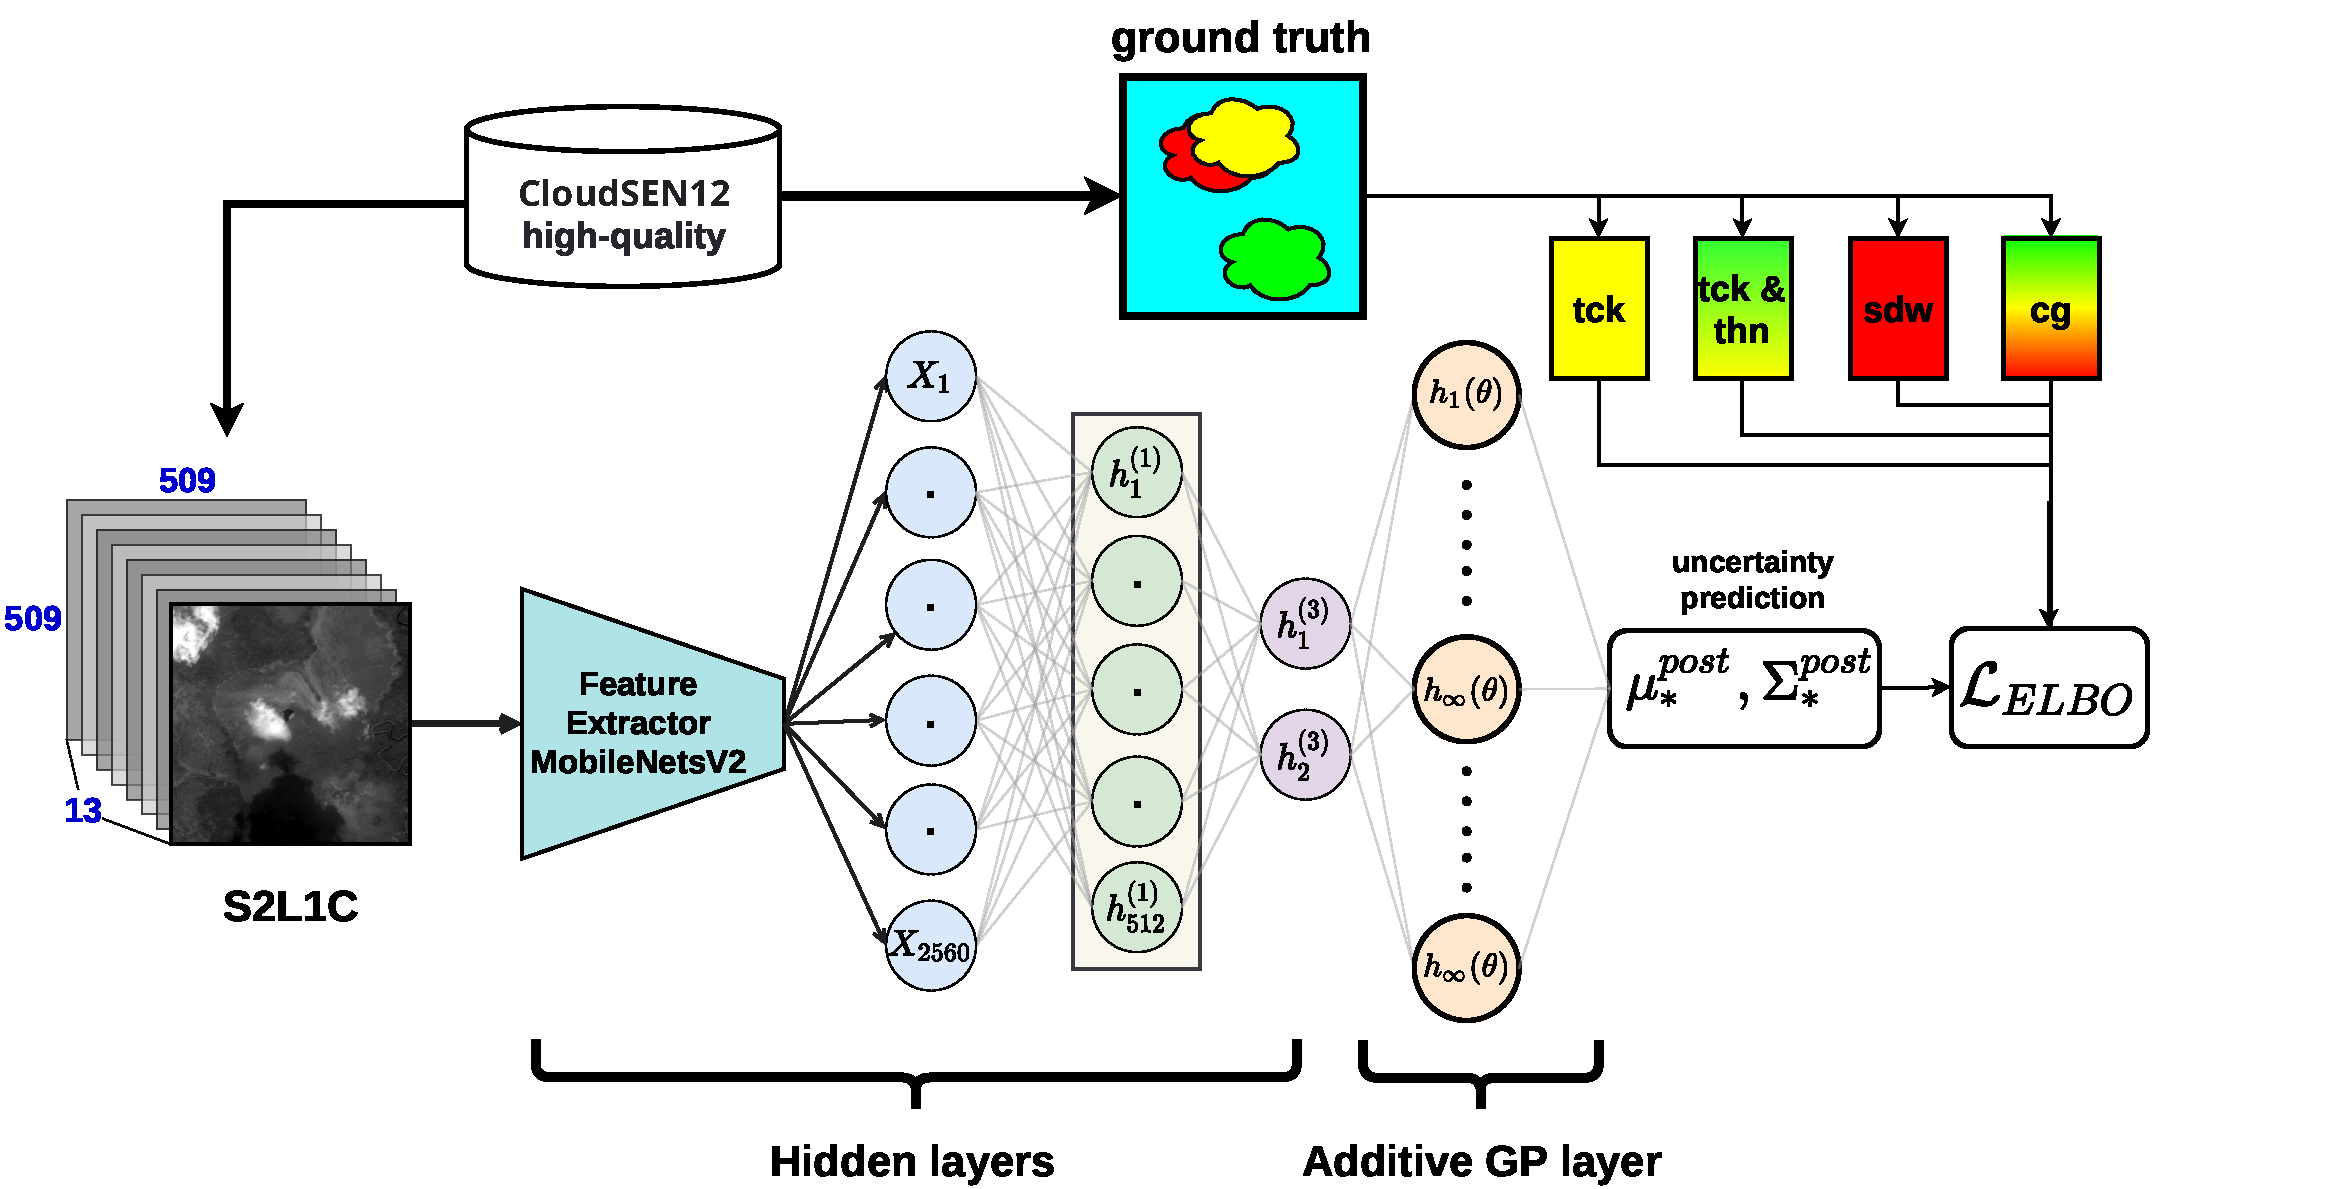
\includegraphics[width=1\linewidth]{images/metodology.pdf}
		\caption{}
		\label{fig:gp01}
	\end{figure}
\end{frame}
